% ------------------------------------------------------------------
\section{Prior Sensitivity and Structural Robustness}
\label{sec:sensitivity}
% ------------------------------------------------------------------
This section stress-tests the conclusions of Sections~\ref{sec:logit}
and~\ref{sec:regression} against four choices made along the way: the prior
variance of the vague model, the global scale of the horseshoe, the treatment
of the ambiguous structural-zero rows, and the size of the training set. Each
check requires a full JAGS refit, so they are run by separate scripts
(\texttt{04a}--\texttt{04d}) whose stored output is read back here.

% ==================================================================
\subsection{Logit model prior sensitivity}
\label{sec:sens-logit}
% ==================================================================
We refit the model of Section~\ref{sec:logit} four times, varying only the
prior variance on every $\beta_j$: $\sigma^2_\beta \in \{1, 10, 100, 10000\}$.
Figure~\ref{fig:prior-sweep} overlays the resulting posterior means and $95\%$
credible intervals, and Table~\ref{tab:prior-range} gives the range each
posterior mean covers across the four fits.

\begin{figure}[htbp]
\centering
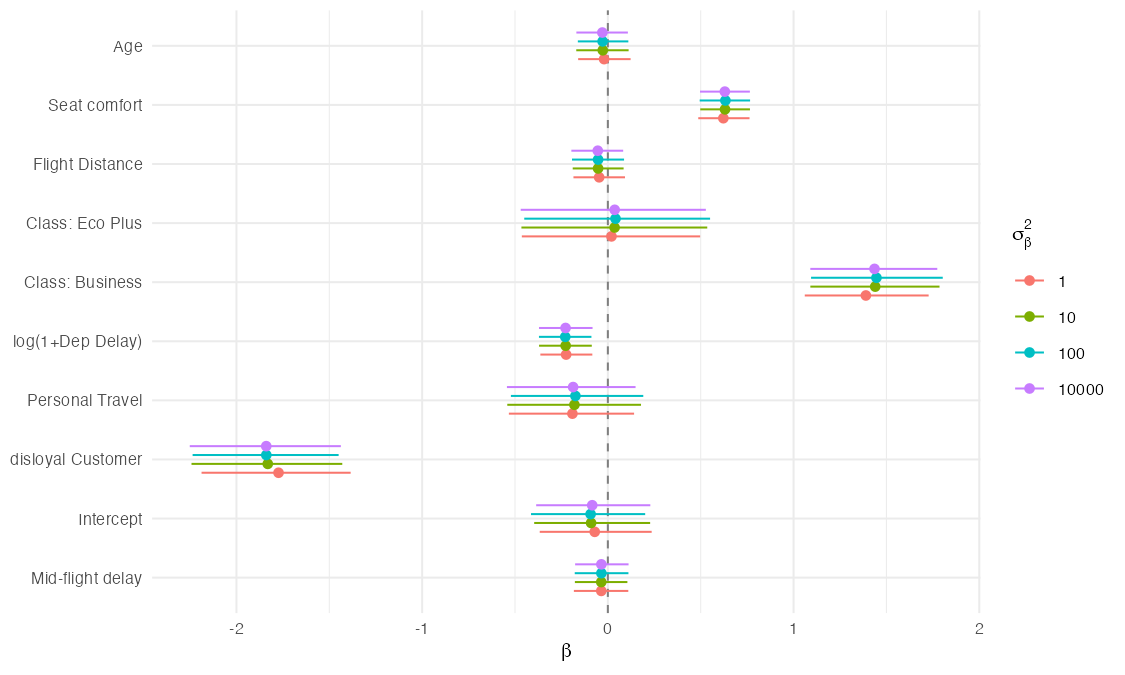
\includegraphics[width=0.85\linewidth]{img/sensitivity/prior_sweep.png}
\caption{Posterior coefficients of the vague-prior logit model across four
prior variances.}
\label{fig:prior-sweep}
\end{figure}

\begin{table}[htbp]
\centering
\caption{Range of posterior means across the four prior variances.}
\label{tab:prior-range}
\begin{tabular}{lc}
\toprule
Term & Range of posterior mean \\
\midrule
disloyal Customer             & 0.066 \\
Class: Business               & 0.057 \\
Intercept                     & 0.022 \\
Class: Eco Plus               & 0.022 \\
Personal Travel               & 0.016 \\
Seat comfort                  & 0.011 \\
Age                           & 0.009 \\
Flight Distance               & 0.008 \\
log(1+Departure Delay)        & 0.005 \\
Mid-flight delay (signed-log) & 0.001 \\
\bottomrule
\end{tabular}
\end{table}

Across four orders of magnitude of prior variance the largest movement is
$0.066$ on the log-odds scale, for a coefficient whose posterior mean is itself
of order $1$--$2$. At $n \approx 1200$ the likelihood dominates every prior we
tested, so the vague-prior results are not an artefact of the variance we
happened to pick.

% ==================================================================
\subsection{Horseshoe prior sensitivity}
\label{sec:sens-horseshoe}
% ==================================================================
The horseshoe's behaviour is governed by the scale $s$ of the half-Cauchy
prior on the global scale, $\tau \sim \mathcal{C}^+(0,s)$: small $s$ pulls
every coefficient towards zero, large $s$ relaxes the shrinkage. It is the one
hyperparameter whose value could plausibly change \emph{which} covariates the
model keeps, so it is the one worth testing. We refit the
Section~\ref{sec:regression} model at $s \in \{0.1, 1, 10\}$, holding the local
scales $\lambda_j$ at $\mathcal{C}^+(0,1)$, and recompute the shrinkage weights
$\kappa_j = 1/(1+\lambda_j^2)$.

\begin{figure}[!ht]
\centering
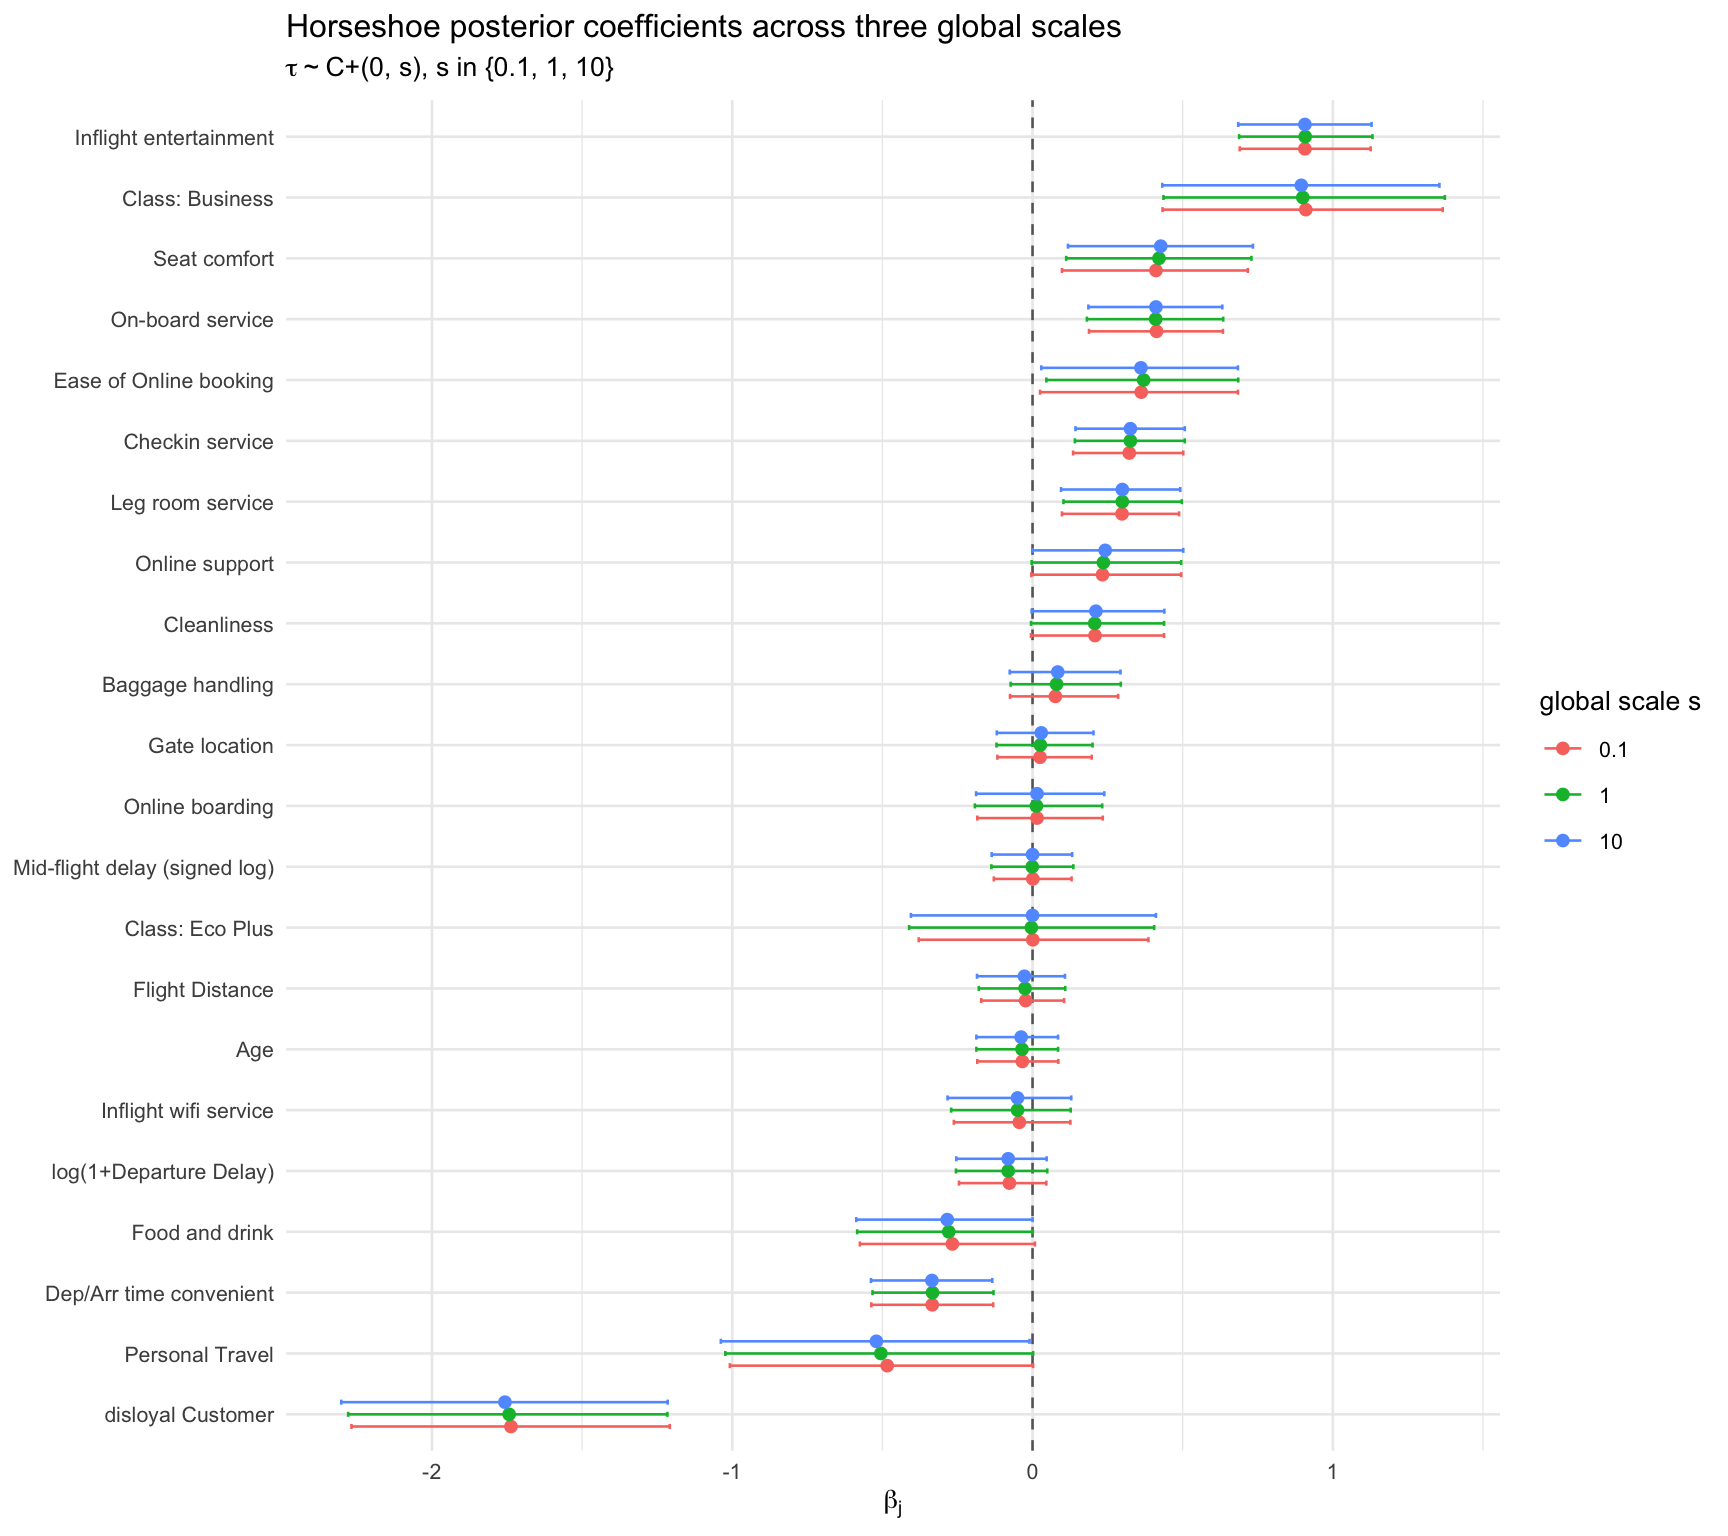
\includegraphics[width=0.62\linewidth]{img/sensitivity/horseshoe_sweep.png}
\caption{Horseshoe posterior coefficients across three global scales, ordered
by shrinkage weight at the default scale.}
\label{fig:hs-beta}
\end{figure}

Across this hundred-fold range exactly one of the $22$ predictors changes its
signal/noise verdict, and no posterior mean moves by more than $0.018$; the
per-predictor weights are tabulated in Appendix~\ref{app:mcmc_horseshoe}. The
strong effects of Section~\ref{sec:regression} remain strong and confidently
non-zero at every scale. What little drift there is sits among coefficients
already on the $\kappa = 0.5$ boundary, which is where sensitivity to $s$ is
expected and where we drew no firm conclusions in the first place.

% ==================================================================
\subsection{Structural-zero robustness check}
\label{sec:sens-structzero}\label{sec:robustness}
% ==================================================================
Section~\ref{sec:regression} raised the possibility that the negative
coefficient on \texttt{Departure/Arrival time convenient} is an artefact of the
structural zeros flagged in Section~\ref{sec:data_expl}, that is, of zeros
meaning ``not applicable'' rather than genuine dissatisfaction. Refitting the
horseshoe model without those rows drops $110$ records and leaves $1103$.

\begin{table}[htbp]
\centering
\caption{Horseshoe refit excluding structural-zero rows. Only the predictors
kept as signal ($\kappa_j < 0.5$) are shown; the full table is in
Appendix~\ref{app:mcmc_horseshoe}.}
\label{tab:structzero}
\begin{tabular}{lcccc}
\toprule
Term & $\beta$ mean & $\beta$ lo & $\beta$ hi & $\kappa_j$ \\
\midrule
Disloyal Customer              & $-2.286$ & $-2.975$ & $-1.599$ & 0.059 \\
Inflight entertainment         & $+1.090$ & $+0.833$ & $+1.361$ & 0.165 \\
Class: Business                & $+0.976$ & $+0.387$ & $+1.535$ & 0.199 \\
Seat comfort                   & $+0.881$ & $+0.577$ & $+1.194$ & 0.209 \\
Personal Travel                & $-0.641$ & $-1.278$ & $-0.008$ & 0.331 \\
On-board service               & $+0.521$ & $+0.231$ & $+0.798$ & 0.338 \\
Dep/Arr time convenient        & $-0.513$ & $-0.782$ & $-0.234$ & 0.347 \\
Ease of Online booking         & $+0.493$ & $+0.090$ & $+0.902$ & 0.370 \\
Checkin service                & $+0.378$ & $+0.154$ & $+0.595$ & 0.420 \\
Leg room service               & $+0.297$ & $+0.056$ & $+0.529$ & 0.486 \\
\bottomrule
\end{tabular}
\end{table}

The hypothesis does not survive. The coefficient does not shrink towards zero
once the ambiguous rows are removed; it becomes \emph{more} negative, from
$-0.335$ to $-0.513$, with a slightly wider interval as expected with $110$
fewer records. Whatever drives the effect, it is not the structural-zero
ambiguity we suspected, and we report it as an open finding rather than force a
tidier story onto it.

The other two members of that correlated cluster move in opposite directions.
\texttt{Seat comfort} strengthens, $\kappa$ falling from $0.367$ to $0.209$ and
$\beta$ rising from $+0.419$ to $+0.881$, while \texttt{Food and drink} goes
from a borderline signal ($\kappa = 0.492$, $\beta = -0.275$) to firmly shrunk
($\kappa = 0.733$, $\beta = +0.020$). The structural zeros therefore do not add
uniform noise across the cluster; they affect its members differently.

% ==================================================================
\subsection{Sample-size robustness}
\label{sec:sens-samplesize}
% ==================================================================
The checks above varied the prior and which rows enter the fit; this one varies
how many. Every model in this report is estimated on \num{1213} records,
following the project brief, which supplies a 1000-customer subset of the
original data for exactly this purpose. Refitting the model of
Section~\ref{sec:logit} on a stratified subsample of \num{15003} records leaves
the coefficients we rely on unmoved, \texttt{Class: Business} by $0.005$,
\texttt{disloyal Customer} by $0.014$ and \texttt{Seat comfort} by $0.022$, and
contracts the credible intervals by a median factor of $3.42$ against the
$3.52$ that $\sqrt{n}$ asymptotics predicts. Three weak effects
(\texttt{Flight Distance}, \texttt{Age}, \texttt{Mid-flight delay}) acquire
intervals excluding zero, which is a limitation of the $n = 1213$ analysis
rather than a finding about the airline.
